% Generated by scripts/2026-10-21/extract_floats.py from paper/main_en.tex; edit the full manuscript, not this file.
\begin{figure}[htbp]
\centering
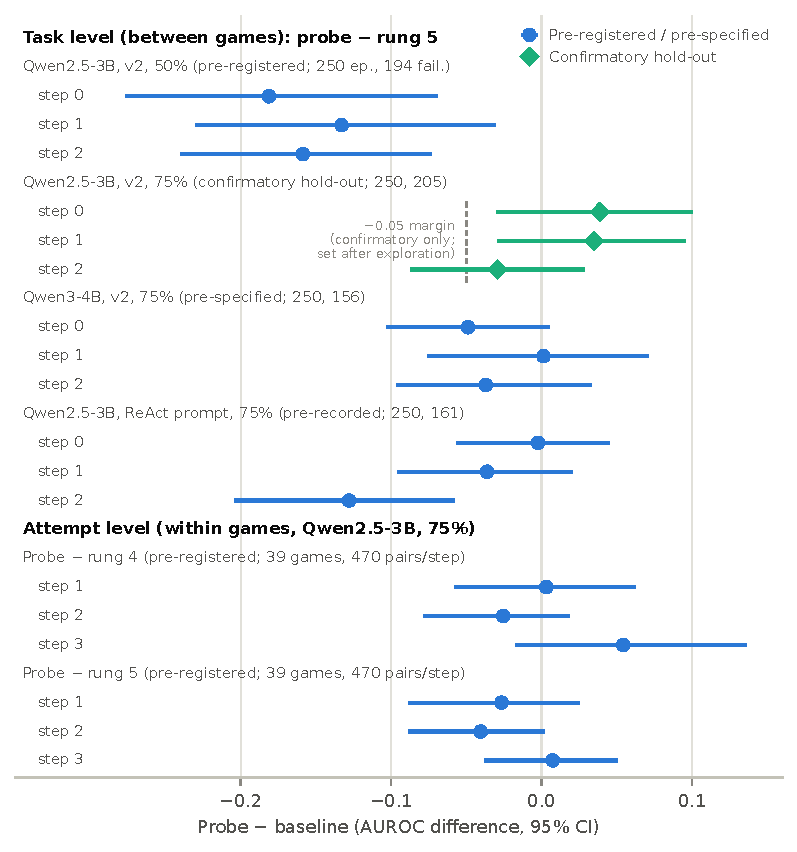
\includegraphics[width=0.82\linewidth]{fig3_probe_minus_baseline.pdf}
\caption{All pre-registered, pre-specified and confirmatory probe-versus-baseline comparisons (18; none superior). Points are AUROC differences with 95\% CIs. Task level: probe $-$ rung 5, scene-level cluster bootstrap (1,000 resamples); labels give the setting and $n$ (episodes, failures). Attempt level: within-game pairwise AUROC differences, game-level bootstrap (1,000 resamples); on label-shuffled data these intervals covered the null value only 80--94\% of the time (Section~\ref{sec:attempt}), so they are too narrow. Dashed segment: $-0.05$ non-inferiority margin, applied only to the confirmatory hold-out and set after the exploratory analysis. Exploratory estimates are not shown (Fig.~\ref{fig:heat}).}\label{fig:forest}
% Sources: results/probe_main_3b_primary_diff.csv, confirm_main_3b_diff.csv, task_qwen3_4b_diff_p.csv, task_react_qwen25_3b_diff_p.csv, within_game_diff.csv
\end{figure}
